\chapter{Robustness study}
\label{chap:robustness}

The numbers reported in \cref{chap:results} all assume that the
deployment distribution matches the training distribution. In
practice, a deployed beacon will see varying noise conditions and
anomaly shapes that the templates do not capture exactly. This chapter
quantifies how gracefully each architecture degrades when the
deployment data is forced \emph{out of distribution} along two
controlled axes.

\section{Protocol}
\label{sec:rob-protocol}

The robustness script
(\texttt{architectures/robustness\_test.py}) generates a series of
small test datasets, each one with $50$ injected events, varying a
single distortion parameter while holding the other at its baseline
value:

\begin{enumerate}[leftmargin=*, itemsep=0.2em]
    \item \textbf{Background-noise sweep.} The high-frequency
    noise standard deviation $\sigma$ is multiplied by
    $m_{\text{noise}} \in \{1.00, 1.22, 1.44, 1.67, 1.89, 2.11, 2.33,
    2.56, 2.78, 3.00\}$. To make the sweep a fair test of
    \emph{absolute} robustness rather than a constant SNR test, the
    target amplitude range of injected anomalies is divided by
    $m_{\text{noise}}$, keeping the absolute strength of the anomaly
    constant.
    \item \textbf{Anomaly-shape-deformation sweep.} The
    deformation-variance parameter $\nu$ of the template generator
    (see \cref{sec:deformation}) is multiplied by
    $m_{\text{deform}} \in \{1.00, 1.78, 2.56, \dots, 8.00\}$ (ten
    evenly-spaced values between $1$ and $8$). Background noise is held
    at its training value.
\end{enumerate}

Each generated dataset is then passed through the trained model and
evaluated with the event-level protocol of \cref{sec:event-eval}. The
metric reported is the macro F1 across the six anomaly classes.

\section{Results}
\label{sec:rob-results}

\Cref{fig:robustness} overlays the three architectures' macro F1
degradation curves on a common scale; the dotted horizontal line marks
the F1 $=50\%$ threshold below which the model is no longer reliably
useful.

\begin{figure}[H]
    \centering
    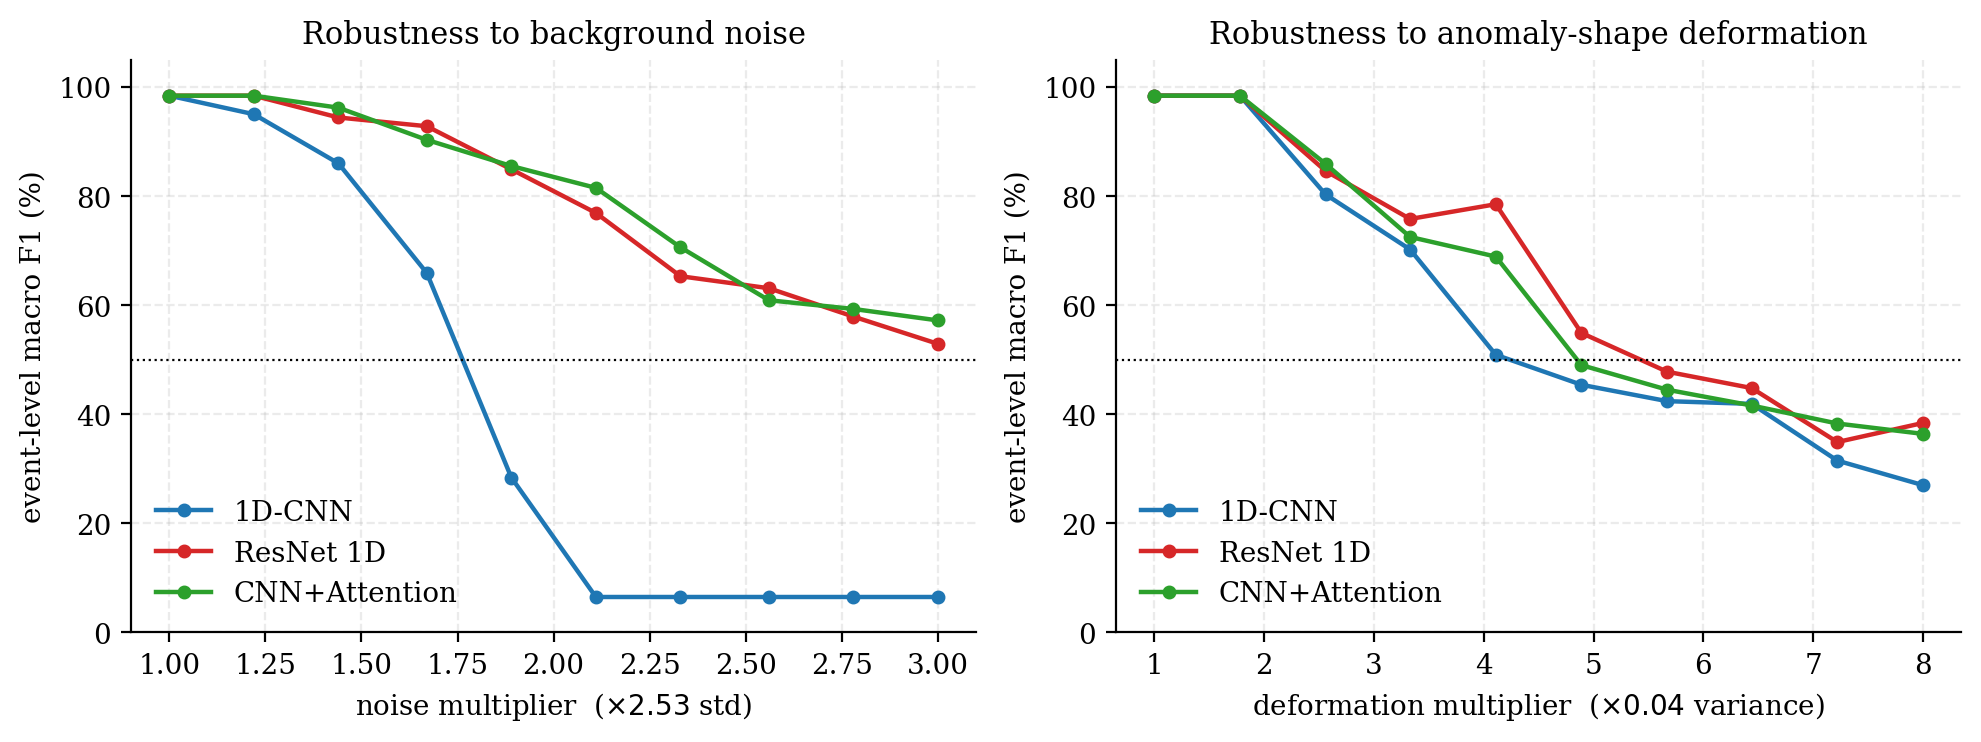
\includegraphics[width=\linewidth]{figures/robustness}
    \caption{Robustness curves. \textbf{Left}: event-level macro F1 as a
    function of the background-noise multiplier. \textbf{Right}: macro
    F1 as a function of the anomaly-shape deformation multiplier. The
    dotted line marks $50\%$ F1.}
    \label{fig:robustness}
\end{figure}

\paragraph{Background-noise sweep.}
\begin{itemize}[leftmargin=*, itemsep=0.2em]
    \item The \textbf{1D-CNN} collapses dramatically: its F1 drops
    below $50\%$ at $m_{\text{noise}} \approx 1.9$ and reaches the
    floor of $\sim 7\%$ already at $m_{\text{noise}} = 2.1$, where the
    model essentially predicts a single class for the entire signal.
    \item The \textbf{ResNet} and the \textbf{CNN+Attention}
    \emph{never} dip below $50\%$ on this sweep --- even at
    $m_{\text{noise}} = 3.0$, where the noise standard deviation is
    three times what the model was trained on, they retain $53\%$ and
    $57\%$ F1 respectively. The two are essentially indistinguishable
    on this axis.
\end{itemize}

\paragraph{Anomaly-shape-deformation sweep.}
\begin{itemize}[leftmargin=*, itemsep=0.2em]
    \item All three models degrade smoothly and only fall below $50\%$
    F1 at deformation multipliers of $\sim 5{-}6$, i.e.\ when the
    keypoint jitter exceeds $20\%{-}30\%$ of the template's normalised
    height --- a level at which a human would also struggle to assign
    a class.
    \item The \textbf{ResNet} is the most resilient to extreme
    deformation, maintaining $\sim 45\%$ F1 up to $m_{\text{deform}}
    = 6.4$ where the other two have dropped below $42\%$. The
    \textbf{CNN+Attention} is essentially on par.
    \item The \textbf{1D-CNN} is the first to break, falling below
    $50\%$ at $m_{\text{deform}} \approx 4.9$.
\end{itemize}

\section{Discussion}
\label{sec:rob-discuss}

Two structural conclusions can be drawn from the robustness study.

\paragraph{1. Residual connections are the single biggest win.}
The gap between the baseline 1D-CNN and the ResNet is enormous on the
noise axis ($\sim 50$ F1 points at $m_{\text{noise}} = 2.0$) and
significant on the deformation axis. The two architectures have an
otherwise identical recipe (same trunk depth, same output head, same
input window). The only differences are (i) residual connections and
(ii) the substitution of BatchNorm by GroupNorm. We can disentangle
these in principle by training a third ablation, but both effects
point in the same direction: a network whose features survive a small
distribution shift is structurally important for an operational
beacon.

\paragraph{2. Self-attention does not buy extra robustness here.}
On both axes the CNN+Attention model is essentially tied with the
ResNet. The Transformer encoder layers add capacity for long-range
reasoning, but the windows in this problem are short ($512$ samples,
$\sim 8.5$ hours), so attention does not have much extra context to
exploit. On a much longer window --- say a $24$-hour window with
several events of interest --- we would expect the attention model to
pull ahead. With the current $W=512$ setup, the attention block
essentially behaves like an additional global-pooling step, and the
extra cost is not amortised.

\paragraph{3. The flat-line failure of the 1D-CNN at high noise.}
The most striking artefact in \cref{fig:robustness} (left) is the
plateau at F1 $\approx 6.5\%$ for the 1D-CNN above $m_{\text{noise}}
= 2.1$. A macro F1 of $6.5\%$ on six classes corresponds approximately
to the model predicting a \emph{single} non-trivial class for the
whole signal: it correctly identifies all the events of that class
(perfect recall) but misses all the others entirely, leaving precision
and recall on the other five classes at zero. This is a hallmark of a
classifier that has lost confidence in its features and falls back to
the largest receptive bias. The same failure mode is the one we will
diagnose on real data in \cref{chap:realdata}.

\paragraph{Operational implications.}
A beacon that operates over years sees seasonal variations in
background noise that easily exceed a $\times 1.5$ multiplier. The
robustness data argue that the residual or attention architecture is
the only viable choice if the system has to keep functioning across
seasons without retraining.
